\documentclass{article}
\usepackage[utf8]{inputenc}
\usepackage{amsmath}
\usepackage{amssymb}
\usepackage{graphicx}

\begin{document}
\section*{Sparse Approximative Inverse}
We are given a regular sparse matrix $\mathbf{A}\in \mathbb{R}^{n,n}$ with $N \in \mathbb{N}$ and at most $n \ll N$ non-zero entries per row and column. We define the space of matrices with the same pattern (on non-zero entries) as $\mathbf{A}$ by
\begin{equation*}
    \mathcal{P}\left(\mathbf{A}\right) := \left\{\mathbf{X} \in \mathbb{R}^{N,N} \: : \: \left(A\right)_{ij} = 0 \implies \left(X\right)_{ij} = 0\right\}
\end{equation*}
We the define the "primitive" sparse approximate inverse (SPAI) $\mathbf{B}$ of $\mathbf{A}$ as
\begin{equation}
    \mathbf{B} := \underset{\mathbf{X}\in \mathcal{P}\left(\mathbf{A}\right)}{\text{argmin}}\left\lVert \mathbf{I}-\mathbf{A}\mathbf{X}\right\rVert_{F}
\end{equation}
here $\left\lVert\:.\:\right\rVert$denotes the Frobenius norm.

\begin{figure}[!hbt]
    \centering
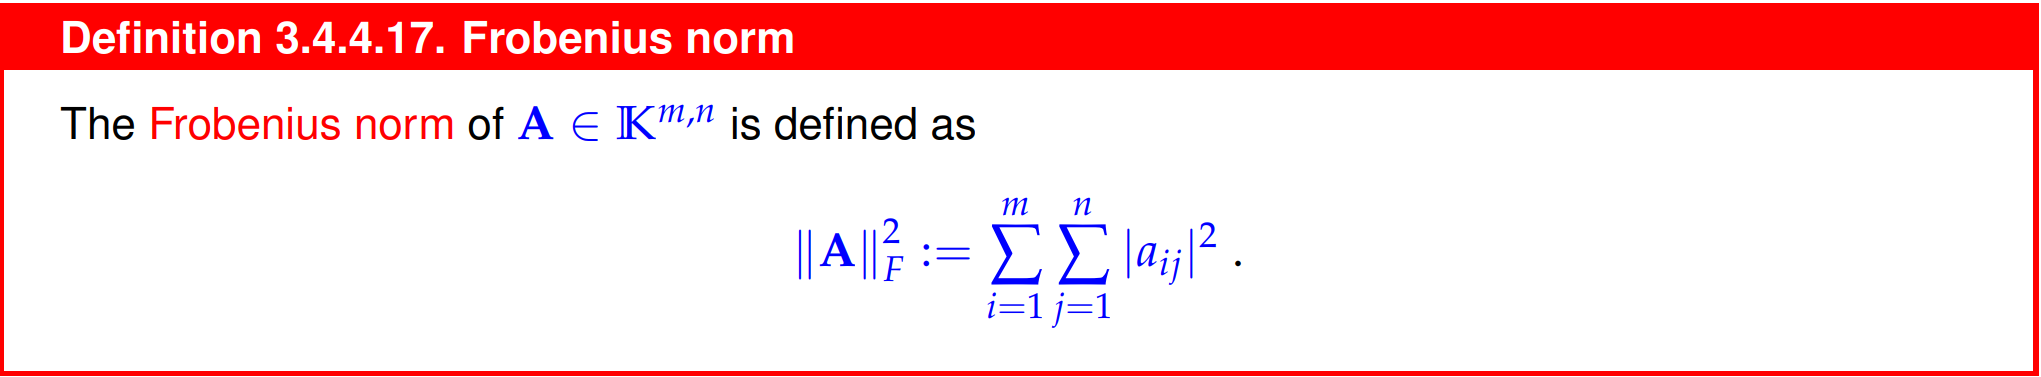
\includegraphics[width=1.0\linewidth]{FrobeniusNorm.png}
\end{figure}

\subsection*{3-6.a} 
We are tasked with showing that the entries of $\mathbf{B}$ can be computed independently of each other by solving linear least squares problems. We first rewrite the Frobenius norm to
\begin{equation*}
    \left\lVert \mathbf{A}\right\rVert_{F}^{2} = \sum_{i=1}^{m}\sum_{j=1}^{n}\left\lvert a_{ij} \right\rvert^{2} =  \sum_{j=1}^{n}\sum_{i=1}^{m}\left\lvert a_{ij} \right\rvert^{2} = \sum_{j=1}^{n}\left(\mathbf{A}\right)_{j}^{\mathsf{T}}\left(\mathbf{A}\right)_{j} = \sum_{j=1}^{n} \left\lVert \left(\mathbf{A}\right)_{j} \right\rVert_{2}^{2}
\end{equation*}
We then notice that $\left(\mathbf{A}\right)_{j}  = \mathbf{A}\mathbf{e}_{j}$, this then produces (we choose different notation to avoid confusion)
\begin{align*}
    \left\lVert \mathbf{M}\right\rVert_{F}^{2} = \sum_{j=1}^{n} \left\lVert\mathbf{M}\mathbf{e}_{j}  \right\rVert_{2}^{2} &\implies \left\lVert \mathbf{I} - \mathbf{A}\mathbf{X}\right\rVert_{F}^{2} = \sum_{i=1}^{N} \left\lVert \left(\mathbf{I}-\mathbf{A}\mathbf{X}\right)\mathbf{e}_{i}\right\rVert_{2}^{2} \\
    &\implies \left\lVert \mathbf{I} - \mathbf{A}\mathbf{X}\right\rVert_{F}^{2} = \sum_{i=1}^{N} \left\lVert \left(\mathbf{e}_{i}-\mathbf{A}\mathbf{X}\mathbf{e}_{i}\right)\right\rVert_{2}^{2} \\
    &\implies \left\lVert \mathbf{I} - \mathbf{A}\mathbf{X}\right\rVert_{F}^{2} = \sum_{i=1}^{N} \left\lVert \left(\mathbf{e}_{i}-\mathbf{A}\left(\mathbf{X}\right)_{i}\right)\right\rVert_{2}^{2} \\
    \end{align*}
Hence we get the following minimization problems
\begin{equation*}
    \mathbf{b}_{i} := \underset{\left(\mathbf{X}\right)_{i} i\text{-th col of } \mathbf{X}\: : \:  \mathbf{X}\in\mathcal{P}\left(\mathbf{A}\right)}{\text{argmin}}\left\lVert \mathbf{e}_{i} - \mathbf{A}\mathbf{X}_{i}\right\rVert_{2} \text{ for } i = 1, \dots , N
\end{equation*}
We did leave away the power of two, as it does not change the result of the minimization, as we are looking for the argument that minimizes the expression and not the minimum of the expression. Let us look at the definition of a linear least squares problem next.
\begin{figure}[!hbt]
    \centering
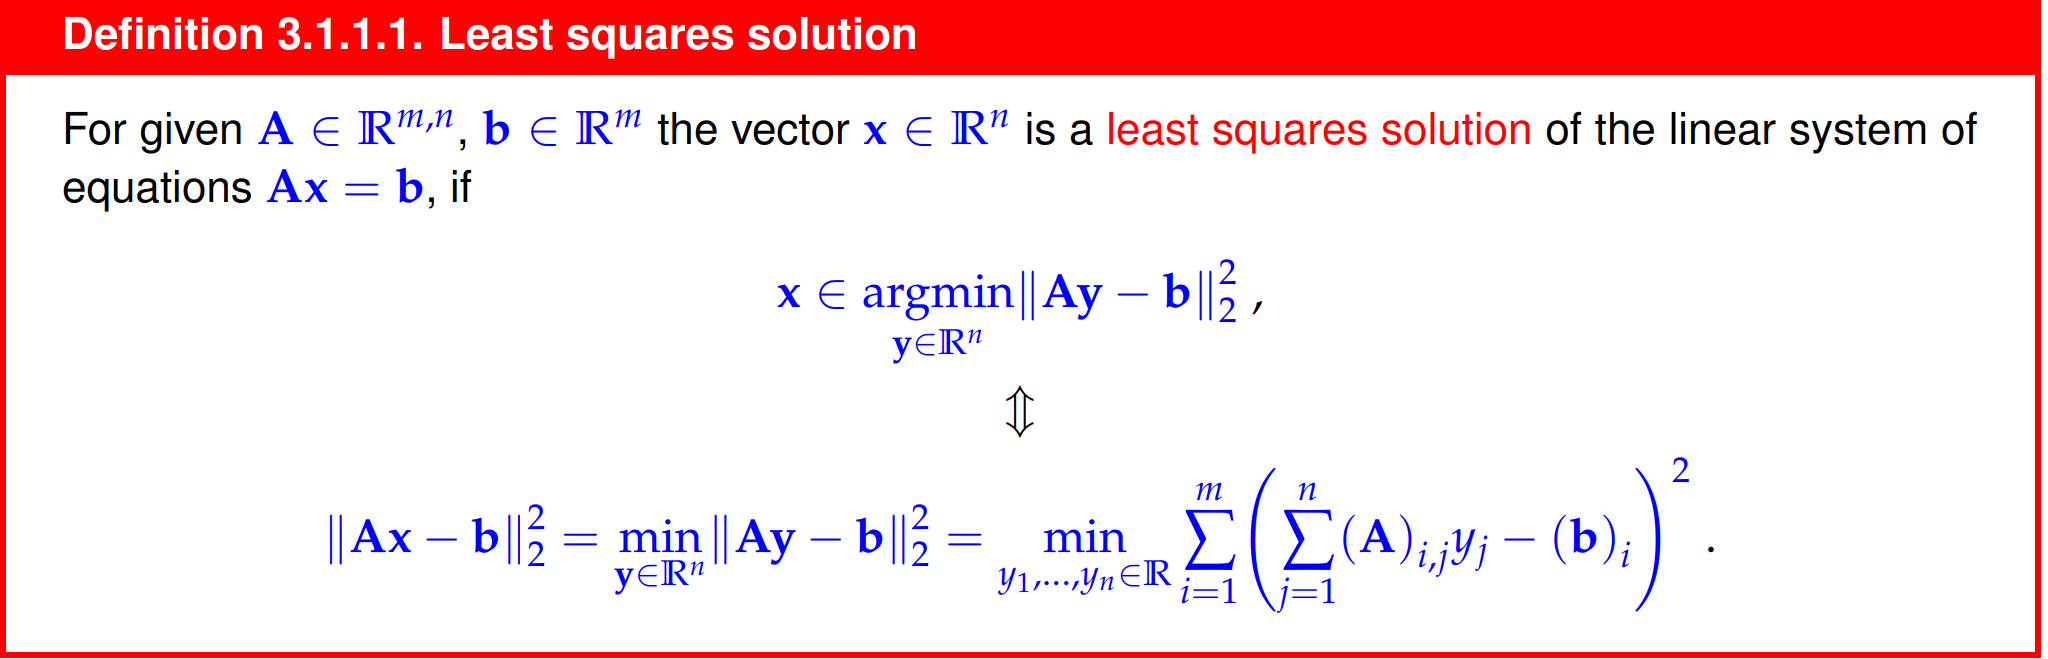
\includegraphics[width=1.0\linewidth]{LinearLeastSquaresDef.png}
\end{figure}

\noindent We can see that our minimization problem is not yet of this form, as we would require all $\mathbf{y}\in \mathbb{R}^{n}$ to be considered instead of only the $\mathbf{y}$ which are columns of matrices in $\mathcal{P}\left(\mathbf{A}\right)$. We remember that we have
\begin{equation*}
    \left(\mathbf{A}\right)_{i,j} = 0 \implies \left(\mathbf{X}\right)_{i,j}  = 0
\end{equation*}
We can hence instead of putting a restriction on $\mathbf{y}$ put a restriction on $\mathbf{A}$. We thus transform
\begin{equation*}
    \mathbf{A}\left(\mathbf{X}\right)_{i}\longrightarrow \mathbf{A}_{i}\mathbf{y}
\end{equation*}
Where by $\mathbf{A}_{i}$ we denote the matrix we get by removing all columns from $\mathbf{A}$ for which 
 the corresponding $\left(\mathbf{X}\right)_{i}$ (the $i$-th column of $\mathbf{X}$) has a zero entry. This makes sense, because as we multiply $\mathbf{A}$ with $\left(\mathbf{X}\right)_{i}$ some columns are never contribute to the result as they are always multiplied with $0$, hence we can preserve the structure of the product by just removing these, we then get a modified minimization problem which is a least squares problem. For this we use some notation that conforms to the solution, we define by $\mathcal{J}$ the set of indices for which $\left(\mathbf{X}\right)_{i}$ has a zero entry, i.e.
 \begin{equation*}
     \mathcal{J} := \left\{j \::\:\left(\mathbf{X}\right)_{i, j} \neq 0 \right\} = \left\{j \::\:\left(\mathbf{A}\right)_{i, j} \neq 0 \right\}
 \end{equation*}
 the equality hold because $\mathbf{X}\in\mathcal{P}\left(\mathbf{A}\right)$. We then proceed to define $m := \left\lvert \mathcal{J}\right\rvert$ and the can finally define $\mathbf{A}_{i}$ as
 \begin{equation*}
     \mathbf{A}_{i} := \left(\mathbf{A}\right)_{:,\mathcal{J}} \in \mathbb{R}^{N,m}
 \end{equation*}
 the set of linear least squares problems is then given by
 \begin{equation*}
      \tilde{\mathbf{b}}_{i} := \underset{\mathbf{y}\in \mathbb{R}^{m}}{\text{argmin}}\left\lVert \mathbf{e}_{i} - \mathbf{A}_{i}\mathbf{y}\right\rVert_{2} \text{ for } i = 1, \dots , N
 \end{equation*}
 We then get the corresponding $\mathbf{b}_{i}$ from adding the zero entries back, as they remain unchanged.
 \subsection*{3-6.b}
 We are tasked with implementing a function for the computation of $\mathbf{B}$. We are allowed to use the built-in linear least squares solver of Eigen. First we must read up on the \verb|SparseMatrix| format in Eigen. Genereally the default is Compressed Column Storage format, however as the Eigen documentation states "A call to the function makeCompressed() turns the matrix into the standard compressed format compatible with many library.", we must make this call to ensure that we are actually working with the compressed column storage format. The following arrays are then defined (we can also define it to be row-major when constructing it)
 \begin{itemize}
    \item\verb|Values|: stores the value of the non-zero entries.
    
\item\verb|InnerIndices|: stores the row indices of the non-zero entries.

     \item\verb|OuterStarts|: stores for each column the index of the first non-zero entry.
     \item\verb|InnerNNZs|: stores the number of non-zeros of each column.
 \end{itemize}
 We also have the following useful methods
 \begin{itemize}
     \item \verb|nonZeros()|: returns the number of non zero coefficients.
     \item\verb|setFromTriplets(iterator begin, iterator end)|: Fills the sparse matrix it is called on with the list of triplets defined by the iterator range begin-end. 
     \item\verb|valuePtr()|: returns a  pointer to the array of values.

     \item\verb|innerIndexPtr()|: returns a  pointer to the array of inner indices.
     \item\verb|outerIndexPtr()|: returns a pointer to the array of the starting positions of the inner vectors.
\end{itemize}
The following utility of \verb|std::vector| may also come in handy
\begin{itemize}
    \item \verb|reserve( amount)|: reserves storage for the specified amount of elements, which does not yet increase the actual size as no elements where added yet.
    \item\verb|emplace(pos, element)|: places the given element into the vector directly \textbf{before} pos (in-place).
    \item\verb|emplace_back(element)|: places a given element in-place at the end.
    \item\verb|push_back|: adds an element to the end
    \item\verb|pop_back|: removes last element
\end{itemize}

\pagebreak

\noindent This gives us the following code, which is pretty unreadable as spacing was removed to allow it to fit onto one page.

\begin{figure}[!hbt]
    \centering
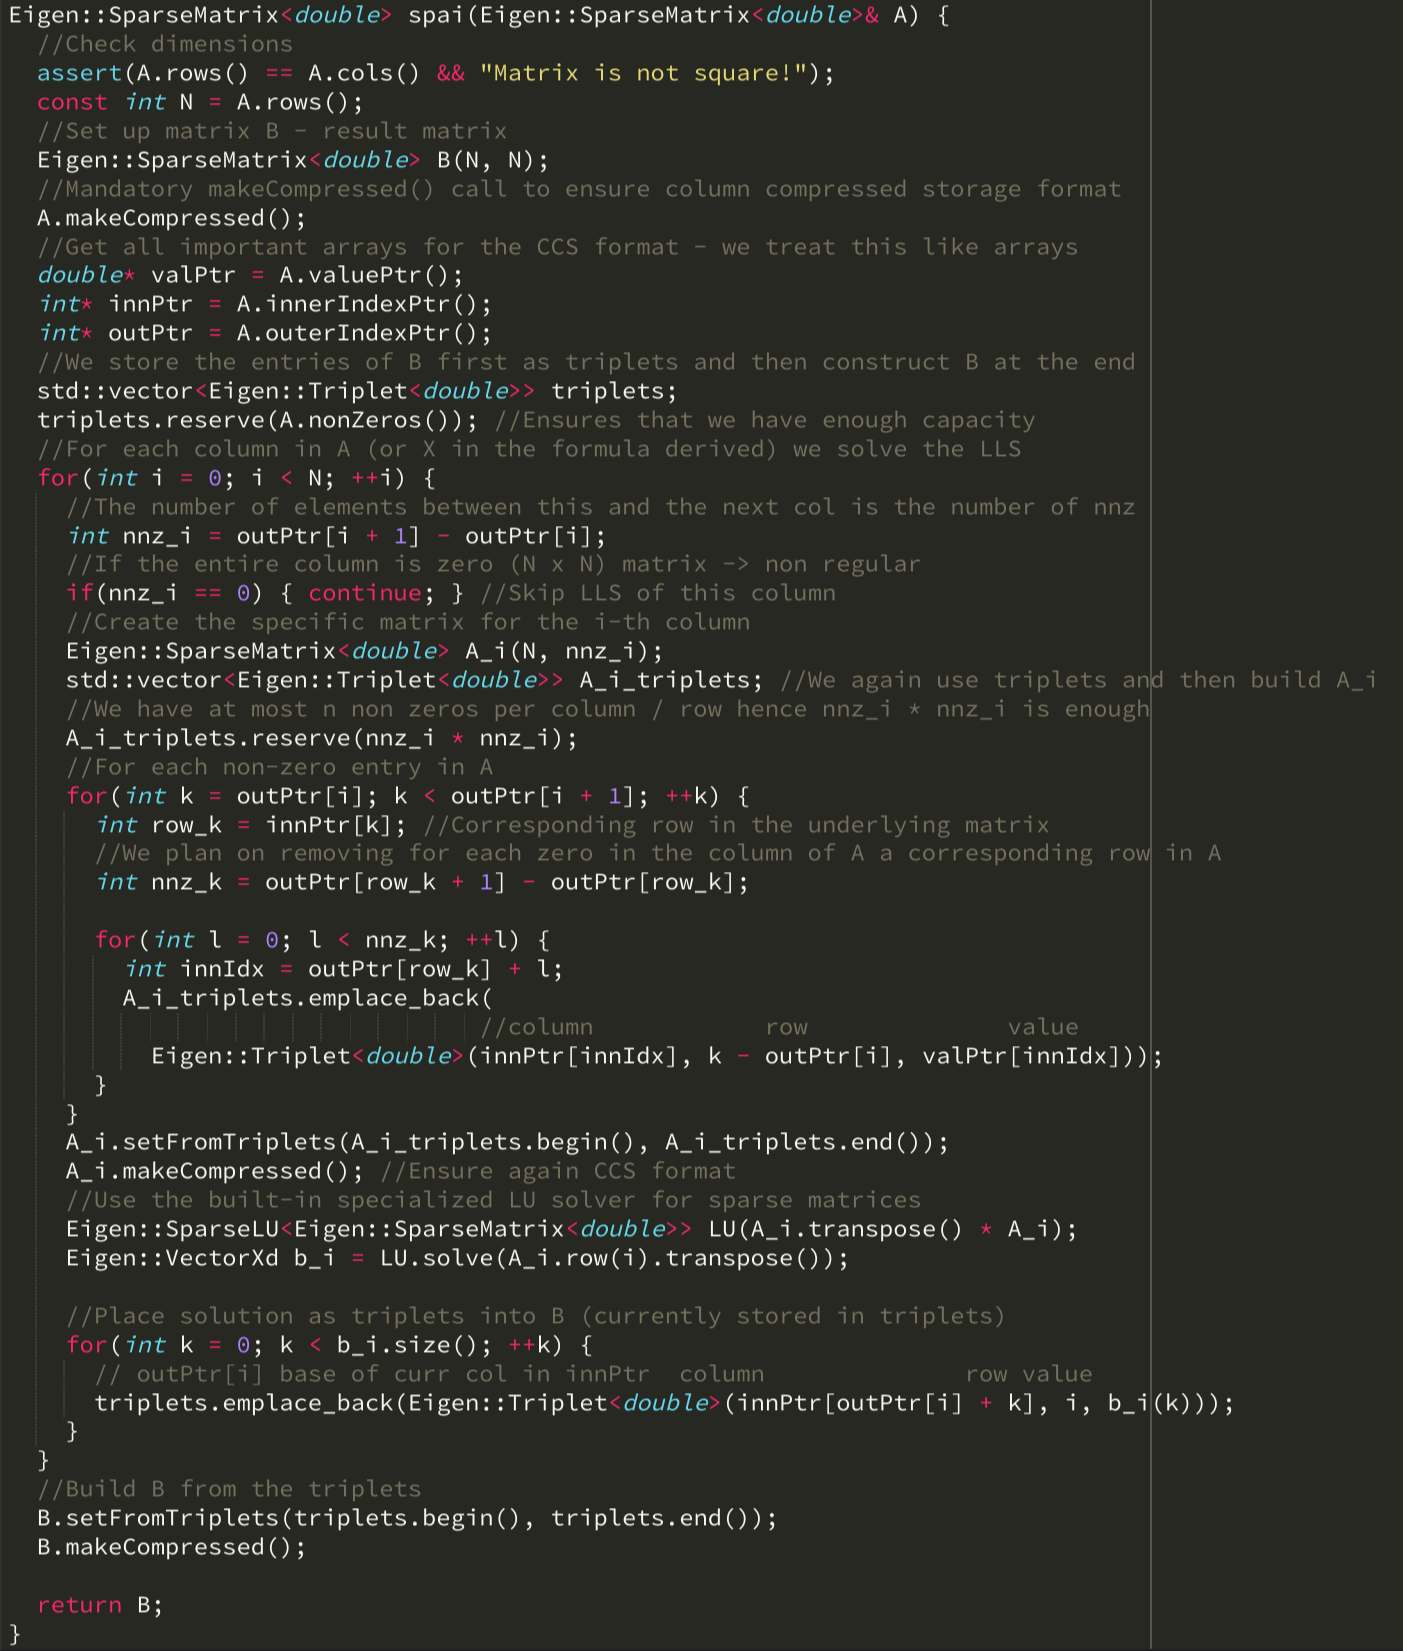
\includegraphics[width=1.0\linewidth]{3-6.b.png}
\end{figure}
\subsection*{3-6.c}
We are tasked with stating the asymptotic computational cost of \verb|spai()|. We have an outer loop doing $N$ iterations, containing an inner loop doing at most $n$ iterations (no more than $n$ non-zeroes per row / column) which itself contains a loop doing at most $n$ iterations (for the same reason). The other expensive operation in the loop is doing LU-decomposition which costs $\mathcal{O}\left(n^{3}\right)$ as $\mathbf{A_{i}}$ is sparse with at most $n$ entries per row / column meaning that $\mathbf{A}_{i}^{\mathsf{T}}\mathbf{A}_{i}$ is of size $\mathcal{O}\left(n^{3}\right)$ and thus both assembly and solving of the system costs $\mathcal{O}\left(n^{3}\right)$. Hence overall we get $\mathcal{O}\left(Nn^{3}\right)$ as we do $n$ iterations that cost $\mathcal{O}\left(n^{3}\right)$ each.
\subsection*{3-6.d}
This was skipped as it relies on knowledge from Chapter 10 which was not discussed.


\end{document}
